\documentclass{article}
\usepackage{tikz}
\usepackage[margin=1in]{geometry}
\begin{document}
\begin{center}
\section*{Graf Podstawowy}
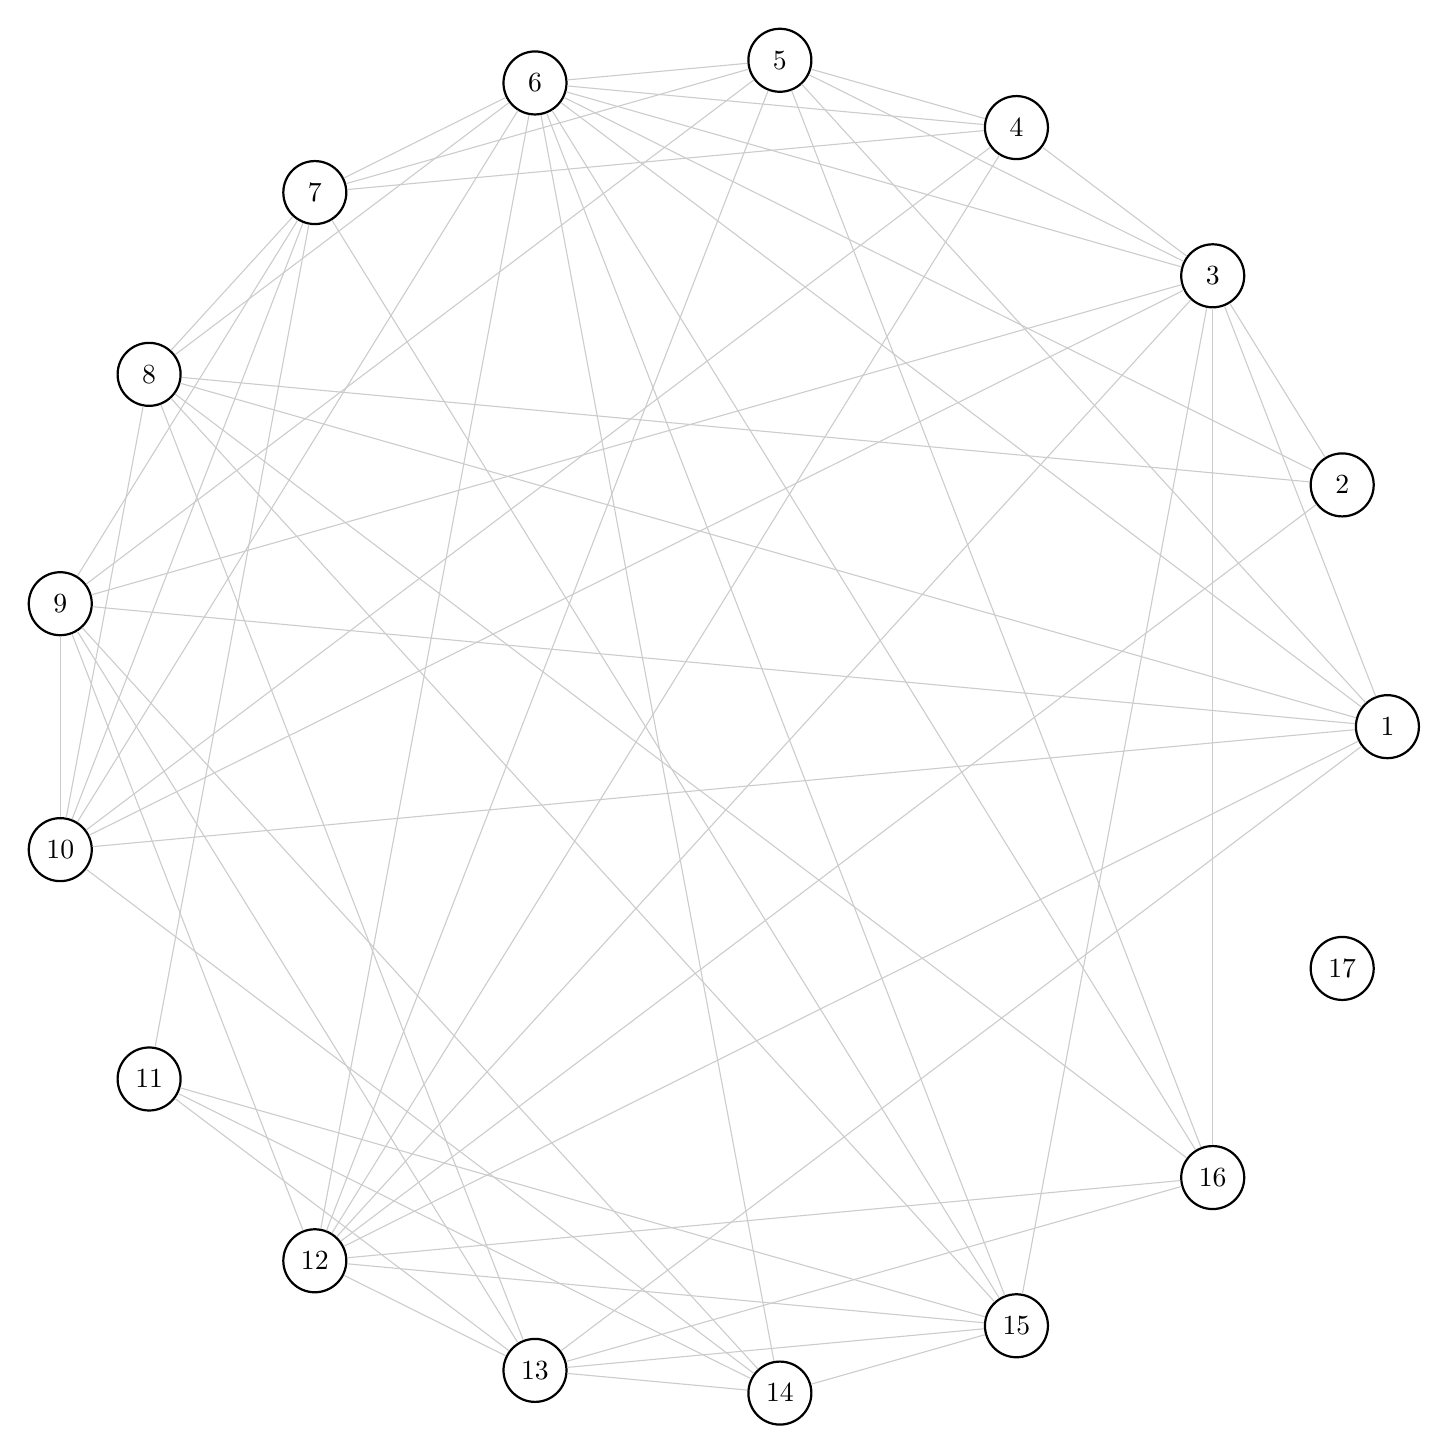
\begin{tikzpicture}[node distance=8.5cm, main/.style = {draw, circle, thick, minimum size=0.8cm, fill=white}, startnode/.style = {draw, circle, ultra thick, minimum size=0.8cm, fill=green!20}]

    % 1. Rozmieszczenie wierzchołków na planie okręgu
    \node[main] (0) at (0.0:8.5) {1};
    \node[main] (1) at (21.176470588235293:8.5) {2};
    \node[main] (2) at (42.35294117647059:8.5) {3};
    \node[main] (3) at (63.529411764705884:8.5) {4};
    \node[main] (4) at (84.70588235294117:8.5) {5};
    \node[main] (5) at (105.88235294117646:8.5) {6};
    \node[main] (6) at (127.05882352941177:8.5) {7};
    \node[main] (7) at (148.23529411764704:8.5) {8};
    \node[main] (8) at (169.41176470588235:8.5) {9};
    \node[main] (9) at (190.58823529411765:8.5) {10};
    \node[main] (10) at (211.76470588235293:8.5) {11};
    \node[main] (11) at (232.94117647058823:8.5) {12};
    \node[main] (12) at (254.11764705882354:8.5) {13};
    \node[main] (13) at (275.29411764705884:8.5) {14};
    \node[main] (14) at (296.4705882352941:8.5) {15};
    \node[main] (15) at (317.6470588235294:8.5) {16};
    \node[main] (16) at (338.8235294117647:8.5) {17};

    % 2. Rysowanie wszystkich krawędzi (na jasnoszaro)
    \draw[gray!40, thin] (0) -- (2);
    \draw[gray!40, thin] (0) -- (4);
    \draw[gray!40, thin] (0) -- (5);
    \draw[gray!40, thin] (0) -- (7);
    \draw[gray!40, thin] (0) -- (8);
    \draw[gray!40, thin] (0) -- (9);
    \draw[gray!40, thin] (0) -- (11);
    \draw[gray!40, thin] (0) -- (12);
    \draw[gray!40, thin] (1) -- (2);
    \draw[gray!40, thin] (1) -- (11);
    \draw[gray!40, thin] (1) -- (5);
    \draw[gray!40, thin] (1) -- (7);
    \draw[gray!40, thin] (2) -- (3);
    \draw[gray!40, thin] (2) -- (4);
    \draw[gray!40, thin] (2) -- (5);
    \draw[gray!40, thin] (2) -- (8);
    \draw[gray!40, thin] (2) -- (9);
    \draw[gray!40, thin] (2) -- (11);
    \draw[gray!40, thin] (2) -- (14);
    \draw[gray!40, thin] (2) -- (15);
    \draw[gray!40, thin] (3) -- (4);
    \draw[gray!40, thin] (3) -- (5);
    \draw[gray!40, thin] (3) -- (6);
    \draw[gray!40, thin] (3) -- (9);
    \draw[gray!40, thin] (3) -- (11);
    \draw[gray!40, thin] (4) -- (5);
    \draw[gray!40, thin] (4) -- (6);
    \draw[gray!40, thin] (4) -- (8);
    \draw[gray!40, thin] (4) -- (11);
    \draw[gray!40, thin] (4) -- (15);
    \draw[gray!40, thin] (5) -- (6);
    \draw[gray!40, thin] (5) -- (7);
    \draw[gray!40, thin] (5) -- (9);
    \draw[gray!40, thin] (5) -- (11);
    \draw[gray!40, thin] (5) -- (13);
    \draw[gray!40, thin] (5) -- (14);
    \draw[gray!40, thin] (5) -- (15);
    \draw[gray!40, thin] (6) -- (7);
    \draw[gray!40, thin] (6) -- (8);
    \draw[gray!40, thin] (6) -- (9);
    \draw[gray!40, thin] (6) -- (10);
    \draw[gray!40, thin] (6) -- (14);
    \draw[gray!40, thin] (7) -- (9);
    \draw[gray!40, thin] (7) -- (12);
    \draw[gray!40, thin] (7) -- (14);
    \draw[gray!40, thin] (7) -- (15);
    \draw[gray!40, thin] (8) -- (9);
    \draw[gray!40, thin] (8) -- (11);
    \draw[gray!40, thin] (8) -- (12);
    \draw[gray!40, thin] (8) -- (13);
    \draw[gray!40, thin] (9) -- (13);
    \draw[gray!40, thin] (10) -- (12);
    \draw[gray!40, thin] (10) -- (13);
    \draw[gray!40, thin] (10) -- (14);
    \draw[gray!40, thin] (11) -- (12);
    \draw[gray!40, thin] (11) -- (14);
    \draw[gray!40, thin] (11) -- (15);
    \draw[gray!40, thin] (12) -- (13);
    \draw[gray!40, thin] (12) -- (14);
    \draw[gray!40, thin] (12) -- (15);
    \draw[gray!40, thin] (13) -- (14);

    % 3. Nakładanie cyklu (pogrubione, kolorowe strzałki)
\end{tikzpicture}
\vspace{1.5cm}

\section*{Cykl Eulera (czerwony)}
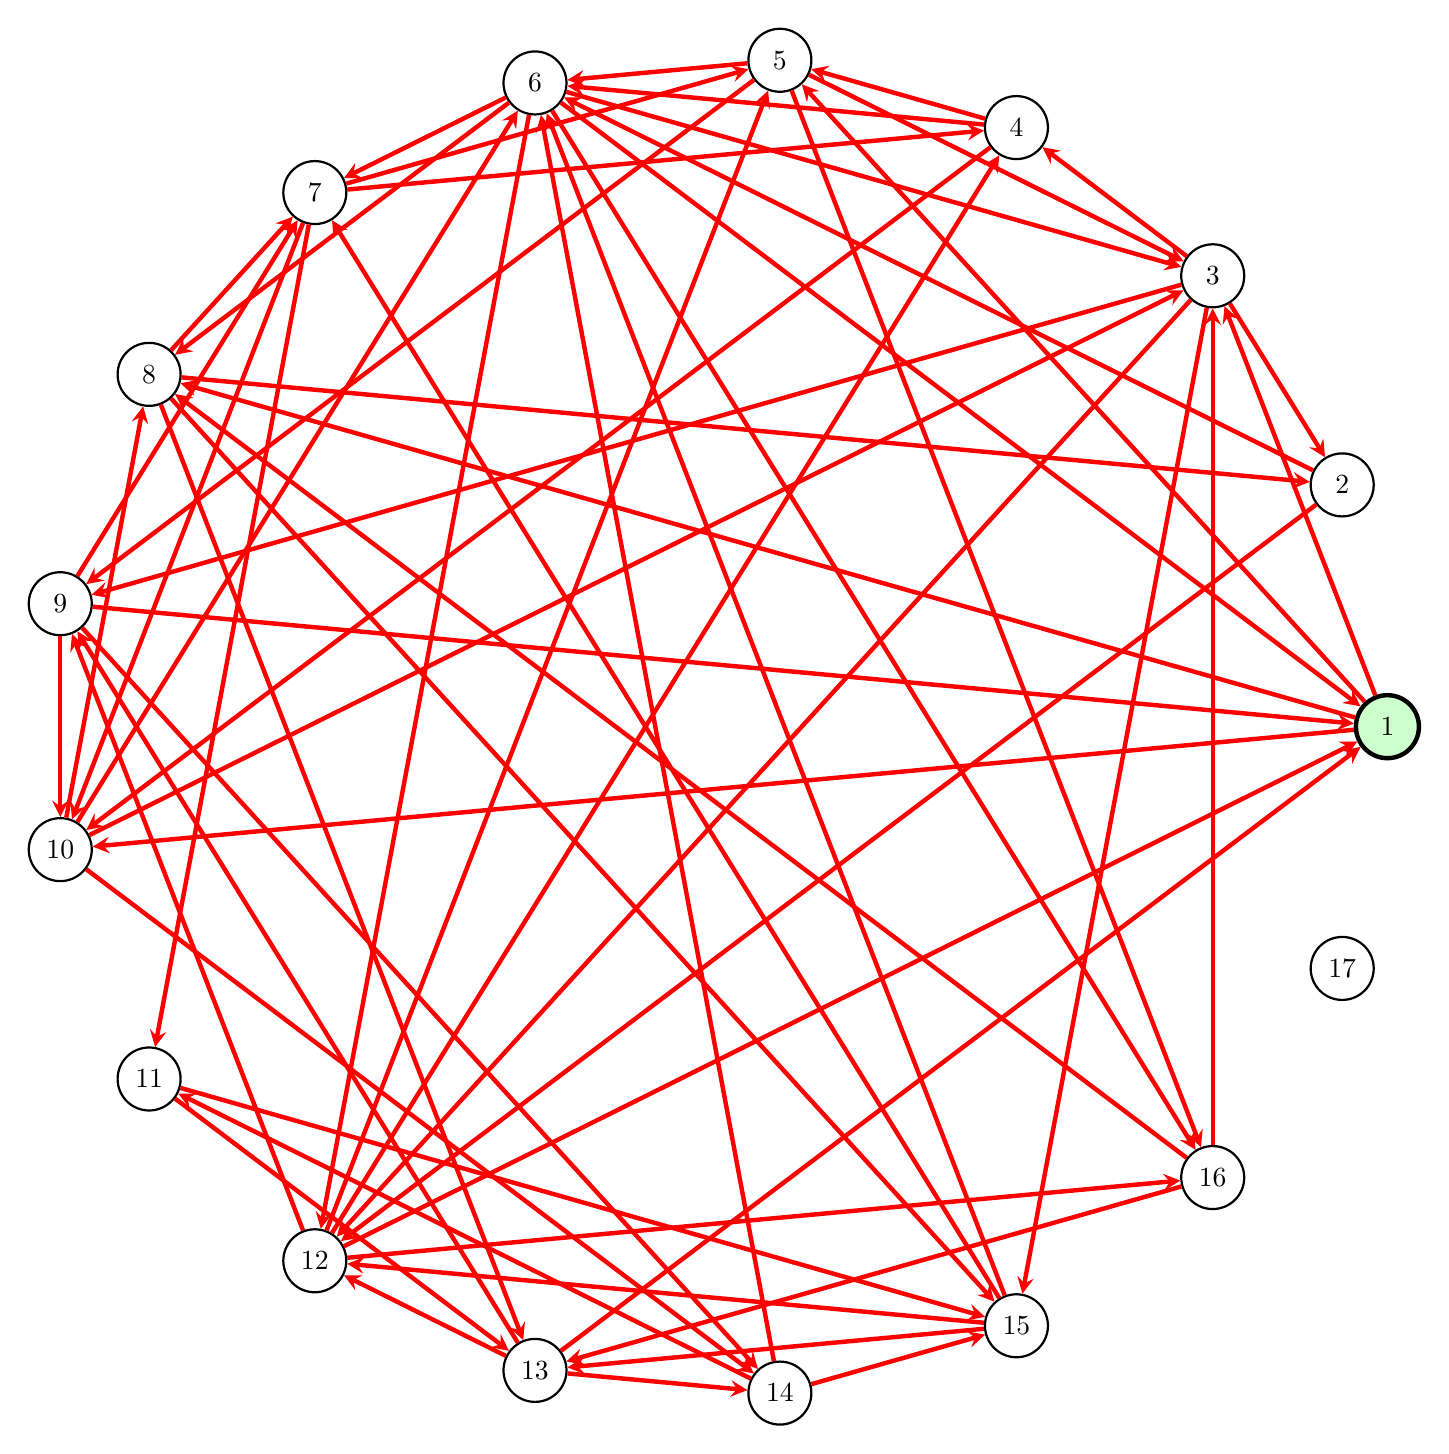
\begin{tikzpicture}[node distance=8.5cm, main/.style = {draw, circle, thick, minimum size=0.8cm, fill=white}, startnode/.style = {draw, circle, ultra thick, minimum size=0.8cm, fill=green!20}]

    % 1. Rozmieszczenie wierzchołków na planie okręgu
    \node[startnode] (0) at (0.0:8.5) {1};
    \node[main] (1) at (21.176470588235293:8.5) {2};
    \node[main] (2) at (42.35294117647059:8.5) {3};
    \node[main] (3) at (63.529411764705884:8.5) {4};
    \node[main] (4) at (84.70588235294117:8.5) {5};
    \node[main] (5) at (105.88235294117646:8.5) {6};
    \node[main] (6) at (127.05882352941177:8.5) {7};
    \node[main] (7) at (148.23529411764704:8.5) {8};
    \node[main] (8) at (169.41176470588235:8.5) {9};
    \node[main] (9) at (190.58823529411765:8.5) {10};
    \node[main] (10) at (211.76470588235293:8.5) {11};
    \node[main] (11) at (232.94117647058823:8.5) {12};
    \node[main] (12) at (254.11764705882354:8.5) {13};
    \node[main] (13) at (275.29411764705884:8.5) {14};
    \node[main] (14) at (296.4705882352941:8.5) {15};
    \node[main] (15) at (317.6470588235294:8.5) {16};
    \node[main] (16) at (338.8235294117647:8.5) {17};

    % 2. Rysowanie wszystkich krawędzi (na jasnoszaro)
    \draw[gray!40, thin] (0) -- (2);
    \draw[gray!40, thin] (0) -- (4);
    \draw[gray!40, thin] (0) -- (5);
    \draw[gray!40, thin] (0) -- (7);
    \draw[gray!40, thin] (0) -- (8);
    \draw[gray!40, thin] (0) -- (9);
    \draw[gray!40, thin] (0) -- (11);
    \draw[gray!40, thin] (0) -- (12);
    \draw[gray!40, thin] (1) -- (2);
    \draw[gray!40, thin] (1) -- (11);
    \draw[gray!40, thin] (1) -- (5);
    \draw[gray!40, thin] (1) -- (7);
    \draw[gray!40, thin] (2) -- (3);
    \draw[gray!40, thin] (2) -- (4);
    \draw[gray!40, thin] (2) -- (5);
    \draw[gray!40, thin] (2) -- (8);
    \draw[gray!40, thin] (2) -- (9);
    \draw[gray!40, thin] (2) -- (11);
    \draw[gray!40, thin] (2) -- (14);
    \draw[gray!40, thin] (2) -- (15);
    \draw[gray!40, thin] (3) -- (4);
    \draw[gray!40, thin] (3) -- (5);
    \draw[gray!40, thin] (3) -- (6);
    \draw[gray!40, thin] (3) -- (9);
    \draw[gray!40, thin] (3) -- (11);
    \draw[gray!40, thin] (4) -- (5);
    \draw[gray!40, thin] (4) -- (6);
    \draw[gray!40, thin] (4) -- (8);
    \draw[gray!40, thin] (4) -- (11);
    \draw[gray!40, thin] (4) -- (15);
    \draw[gray!40, thin] (5) -- (6);
    \draw[gray!40, thin] (5) -- (7);
    \draw[gray!40, thin] (5) -- (9);
    \draw[gray!40, thin] (5) -- (11);
    \draw[gray!40, thin] (5) -- (13);
    \draw[gray!40, thin] (5) -- (14);
    \draw[gray!40, thin] (5) -- (15);
    \draw[gray!40, thin] (6) -- (7);
    \draw[gray!40, thin] (6) -- (8);
    \draw[gray!40, thin] (6) -- (9);
    \draw[gray!40, thin] (6) -- (10);
    \draw[gray!40, thin] (6) -- (14);
    \draw[gray!40, thin] (7) -- (9);
    \draw[gray!40, thin] (7) -- (12);
    \draw[gray!40, thin] (7) -- (14);
    \draw[gray!40, thin] (7) -- (15);
    \draw[gray!40, thin] (8) -- (9);
    \draw[gray!40, thin] (8) -- (11);
    \draw[gray!40, thin] (8) -- (12);
    \draw[gray!40, thin] (8) -- (13);
    \draw[gray!40, thin] (9) -- (13);
    \draw[gray!40, thin] (10) -- (12);
    \draw[gray!40, thin] (10) -- (13);
    \draw[gray!40, thin] (10) -- (14);
    \draw[gray!40, thin] (11) -- (12);
    \draw[gray!40, thin] (11) -- (14);
    \draw[gray!40, thin] (11) -- (15);
    \draw[gray!40, thin] (12) -- (13);
    \draw[gray!40, thin] (12) -- (14);
    \draw[gray!40, thin] (12) -- (15);
    \draw[gray!40, thin] (13) -- (14);

    % 3. Nakładanie cyklu (pogrubione, kolorowe strzałki)
    \draw[red, ultra thick, ->, >=stealth] (0) -- (2);
    \draw[red, ultra thick, ->, >=stealth] (2) -- (1);
    \draw[red, ultra thick, ->, >=stealth] (1) -- (11);
    \draw[red, ultra thick, ->, >=stealth] (11) -- (0);
    \draw[red, ultra thick, ->, >=stealth] (0) -- (4);
    \draw[red, ultra thick, ->, >=stealth] (4) -- (2);
    \draw[red, ultra thick, ->, >=stealth] (2) -- (3);
    \draw[red, ultra thick, ->, >=stealth] (3) -- (4);
    \draw[red, ultra thick, ->, >=stealth] (4) -- (5);
    \draw[red, ultra thick, ->, >=stealth] (5) -- (0);
    \draw[red, ultra thick, ->, >=stealth] (0) -- (7);
    \draw[red, ultra thick, ->, >=stealth] (7) -- (1);
    \draw[red, ultra thick, ->, >=stealth] (1) -- (5);
    \draw[red, ultra thick, ->, >=stealth] (5) -- (2);
    \draw[red, ultra thick, ->, >=stealth] (2) -- (8);
    \draw[red, ultra thick, ->, >=stealth] (8) -- (0);
    \draw[red, ultra thick, ->, >=stealth] (0) -- (9);
    \draw[red, ultra thick, ->, >=stealth] (9) -- (2);
    \draw[red, ultra thick, ->, >=stealth] (2) -- (11);
    \draw[red, ultra thick, ->, >=stealth] (11) -- (3);
    \draw[red, ultra thick, ->, >=stealth] (3) -- (5);
    \draw[red, ultra thick, ->, >=stealth] (5) -- (6);
    \draw[red, ultra thick, ->, >=stealth] (6) -- (3);
    \draw[red, ultra thick, ->, >=stealth] (3) -- (9);
    \draw[red, ultra thick, ->, >=stealth] (9) -- (5);
    \draw[red, ultra thick, ->, >=stealth] (5) -- (7);
    \draw[red, ultra thick, ->, >=stealth] (7) -- (6);
    \draw[red, ultra thick, ->, >=stealth] (6) -- (4);
    \draw[red, ultra thick, ->, >=stealth] (4) -- (8);
    \draw[red, ultra thick, ->, >=stealth] (8) -- (6);
    \draw[red, ultra thick, ->, >=stealth] (6) -- (9);
    \draw[red, ultra thick, ->, >=stealth] (9) -- (7);
    \draw[red, ultra thick, ->, >=stealth] (7) -- (12);
    \draw[red, ultra thick, ->, >=stealth] (12) -- (8);
    \draw[red, ultra thick, ->, >=stealth] (8) -- (9);
    \draw[red, ultra thick, ->, >=stealth] (9) -- (13);
    \draw[red, ultra thick, ->, >=stealth] (13) -- (5);
    \draw[red, ultra thick, ->, >=stealth] (5) -- (11);
    \draw[red, ultra thick, ->, >=stealth] (11) -- (4);
    \draw[red, ultra thick, ->, >=stealth] (4) -- (15);
    \draw[red, ultra thick, ->, >=stealth] (15) -- (2);
    \draw[red, ultra thick, ->, >=stealth] (2) -- (14);
    \draw[red, ultra thick, ->, >=stealth] (14) -- (5);
    \draw[red, ultra thick, ->, >=stealth] (5) -- (15);
    \draw[red, ultra thick, ->, >=stealth] (15) -- (7);
    \draw[red, ultra thick, ->, >=stealth] (7) -- (14);
    \draw[red, ultra thick, ->, >=stealth] (14) -- (6);
    \draw[red, ultra thick, ->, >=stealth] (6) -- (10);
    \draw[red, ultra thick, ->, >=stealth] (10) -- (12);
    \draw[red, ultra thick, ->, >=stealth] (12) -- (11);
    \draw[red, ultra thick, ->, >=stealth] (11) -- (8);
    \draw[red, ultra thick, ->, >=stealth] (8) -- (13);
    \draw[red, ultra thick, ->, >=stealth] (13) -- (10);
    \draw[red, ultra thick, ->, >=stealth] (10) -- (14);
    \draw[red, ultra thick, ->, >=stealth] (14) -- (11);
    \draw[red, ultra thick, ->, >=stealth] (11) -- (15);
    \draw[red, ultra thick, ->, >=stealth] (15) -- (12);
    \draw[red, ultra thick, ->, >=stealth] (12) -- (13);
    \draw[red, ultra thick, ->, >=stealth] (13) -- (14);
    \draw[red, ultra thick, ->, >=stealth] (14) -- (12);
    \draw[red, ultra thick, ->, >=stealth] (12) -- (0);
\end{tikzpicture}
\vspace{1.5cm}

\end{center}
\end{document}
